%% Bookheader, Nov 8, 2020; July 18, 2022

\documentclass[11pt]{../Support/ourbook}
%% or for landscape, comment out line above and use this one:
%%\documentclass[landscape,11pt]{ourbook}

%% This will keep space from stretching around display math:

\makeatletter
\renewcommand\normalsize{%
   \@setfontsize\normalsize\@xipt{13.6}%
   \abovedisplayskip 11\p@  \@minus6\p@
   \abovedisplayshortskip \z@ 
   \belowdisplayshortskip 6.5\p@ \@minus3\p@
   \belowdisplayskip \abovedisplayskip
   \let\@listi\@listI}
\makeatother
\normalsize


\begin{document}

\tableofcontents
\graphicspath{{../../Chapters/angles/en_US}}
\chapter{Angles}

In the following recommend videos, the narrator talks about
lines, line segments, and rays. When mathematicians talk about
\emph{lines}\index{lines}, they mean a straight line that goes forever in two 
directions. And if you pick any two points on that line; the space between 
them is a \emph{line segment}\index{line segment}. If you take any line, pick 
a point on that line and discard all the points on one side of the point, that 
is a \emph{ray}\index{ray}. All three have no width.

\begin{center}
\begin{tikzpicture}[scale=1.5]
  \coordinate (a) at (-0.3, -0.6);
  \coordinate (d) at (1.3, 2.6);
  \draw [<->](a)--node [right]{"Line"}(d);
\end{tikzpicture}
\hspace{10mm}
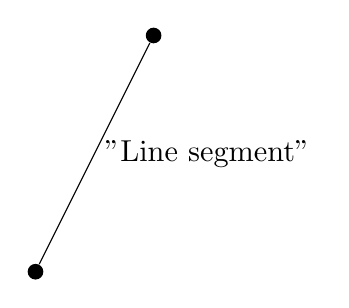
\begin{tikzpicture}[scale=1.5]
  \coordinate [circle, fill, inner sep=2pt] (b) at (0,0) ;
  \coordinate [circle, fill, inner sep=2pt] (c) at (1, 2) ;
  \draw (b)--node [right]{"Line segment"}(c);
\end{tikzpicture}
\hspace{6mm}
\begin{tikzpicture}[scale=1.5]
  \coordinate [circle, fill, inner sep=2pt] (b) at (0,0) ;
  \coordinate (d) at (1.3, 2.6);
  \coordinate (lab) at (0.8, 1.0);
  \draw [->](b)--node[right] {"Ray"} (d)  ;
\end{tikzpicture}
\end{center}



Watch the following videos from Khan Academy:
\begin{itemize}
\item Introduction to angles: \url{https://youtu.be/H-de6Tkxej8}
\item Measuring angles in degrees: \url{https://youtu.be/92aLiyeQj0w} 
\end{itemize}

When two lines cross, they form four angles:

\begin{center}
\begin{tikzpicture}[scale=3]
  \coordinate (a) at (0, 1.5);
  \coordinate (b) at (1.6, 2);
  \coordinate (c) at (1.6, 1.5);
  \coordinate (d) at (0, 1);
  \coordinate [circle, fill, inner sep=1pt](e) at (0.8, 1.5) ;
  \draw [->](e)--(a) node[left] {$A$}  ;
  \draw [->](e)--(b) node[right] {$B$}  ;
  \draw [->](e)--(c) node[right] {$C$}  ;
  \draw [->](e)node[above]{$E$}--(d) node[left] {D} ;
  \pic [draw, <->, "$\scriptstyle  \angle AEB$ ", angle radius = 0.8cm, 
  angle eccentricity=1.3] {angle = b--e--a};
  \pic [draw, <->, "$\scriptstyle  \angle BEC$ ", angle radius = 1.1cm, 
  angle eccentricity = 1.5] {angle = c--e--b};
  \pic [draw, <->, "$\scriptstyle  \angle CED$ ", angle radius = 0.8cm, 
  angle eccentricity=1.3] {angle = d--e--c};
  \pic [draw, <->, "$\scriptstyle  \angle DEA$ ", angle radius = 1.1cm, 
  angle eccentricity=1.5] {angle = a--e--d};
\end{tikzpicture}
\end{center}


What do we know about those angles?
\begin{itemize}
\item The sum of any two adjacent angles add to be $180^\circ$.  So, for 
example, $m \angle AEB + m \angle BEC = 180^\circ$. We use the phrase ``add to 
be $180^{\circ}$'' so often that we have a special word for it: 
\emph{supplementary}.\index{supplementary angles}
\item The sum of all four angles is $360^\circ$.
\item Angles opposite each other are equal. So, for example, $m \angle AEB = m 
\angle CED$.
\end{itemize}

In a diagram, to indicate that two angles are equal we often put hash marks in 
the angle:

\begin{center}
\begin{tikzpicture}[scale=3]
  \coordinate (a) at (0, 1.5);
  \coordinate (b) at (1.6, 2);
  \coordinate (c) at (1.6, 1.5);
  \coordinate (d) at (0, 1);
  \coordinate [circle, fill, inner sep=1pt](e) at (0.8, 1.5) ;
  \draw [->](e)--(a) node[left] {$A$}  ;
  \draw [->](e)--(b) node[right] {$B$}  ;
  \draw [->](e)--(c) node[right] {$C$}  ;
  \draw [->](e)node[above]{$E$}--(d) node[left] {D} ;
  \tkzMarkAngle[size = 0.2cm,mark = |](b,e,a)
  \tkzMarkAngle[size = 0.3cm,mark = ||](c,e,b)
  \tkzMarkAngle[size = 0.2cm,mark = |](d,e,c)
  \tkzMarkAngle[size = 0.3cm,mark = ||](a,e,d)
\end{tikzpicture}
\end{center}


Here the two angles with a single hash mark are equal and the two angles with 
double hash marks are equal.

When two lines are perpendicular, the angle between them is $90^\circ$ and we 
say they meet at a \emph{right angle}. When drawing diagrams, we indicate right
angles with an elbow:

\begin{center}
\begin{tikzpicture}[scale=1.5]
  \coordinate (a) at (0, 1.5);
  \coordinate (b) at (0, 0);
  \coordinate (c) at (1.5, 0);
  \draw [->](b)--(a)  ;
  \draw [->](b)--(c)  ;
  \pic [draw,thick,angle eccentricity=.5]{right angle = a--b--c};
\end{tikzpicture}
\end{center}

 
When an angle is less than $90^\circ$, it is said to be
\emph{acute}. When an angle is more than $90^\circ$, it is said to be
\emph{obtuse}.
% Add: Complementary Angles

\begin{center}
\begin{tikzpicture}[scale=3]
  \coordinate (a) at (0.4, 0.6);
  \coordinate (b) at (0, 0);
  \coordinate (c) at (0.9, 0);
  \draw [->](b)--(a)  ;
  \draw [->](b)--(c)  ;
  \pic [draw, <->, "acute", angle radius = 1cm, angle eccentricity=1.5] {
  angle = c--b--a};
  \end{tikzpicture}
\hspace{2cm}
\begin{tikzpicture}[scale=3]
  \coordinate (a) at (1, 0.6);
  \coordinate (b) at (0.5, 0);
  \coordinate (c) at (0, 0);
  \draw [->](b)--(a)  ;
  \draw [->](b)--(c)  ;
  \pic [draw, <->, "obtuse", angle radius = 0.6cm, angle eccentricity=1.5] {
  angle = a--b--c};
\end{tikzpicture}
\end{center}


If two lines are parallel, line segments that intersect both lines, form the 
same angles with each line:

\begin{center}
\begin{tikzpicture}[scale=3]
  \coordinate (a) at (0, 1);
  \coordinate [circle, fill, inner sep=1pt](b) at (1.5, 1.5);
  \coordinate (c) at (1.5, 1);
  \coordinate (d) at (0.5, 0.5);
  \coordinate (e) at (1, 1);
  \coordinate (f) at (0, 0.5);
  \coordinate (g) at (1.5, 0.5);
  \coordinate [circle, fill, inner sep=1pt](h) at (0, 0);
  \draw [->](e)--(a);
  \draw [-](e)--(b);
  \draw [->](e)--(c);
  \draw [-](e)--(d);
   \draw [->](d)--(f);
  \draw [->](d)--(g);
  \draw [-](d)--(h);
  \tkzMarkAngle[size = 0.15cm,mark = |](b,e,a)
  \tkzMarkAngle[size = 0.2cm,mark = ||](c,e,b)
  \tkzMarkAngle[size = 0.15cm,mark = |](d,e,c)
  \tkzMarkAngle[size = 0.2cm,mark = ||](a,e,d)
  
   \tkzMarkAngle[size = 0.15cm,mark = |](e,d,f)
  \tkzMarkAngle[size = 0.2cm,mark = ||](g,d,e)
  \tkzMarkAngle[size = 0.15cm,mark = |](h,d,g)
  \tkzMarkAngle[size = 0.2cm,mark = ||](f,d,h)
\end{tikzpicture}
\end{center}


\section{Radians}
As you've seen above, angles can be measured in degrees. Just like you can 
measure length in more than one unit (inches, meters, etc.), there is more 
than one unit to measure angles in. Angles can also be measured in \textit{
radians}\index{radians}. Radians are unitless (that is, you don't have to put 
a letter after the number) and there are $\pi$ radians across a straight line. 
This means $180^\circ$ is the same as $\pi$ radians. 

\textbf{Example}: An angle is measured to be $\frac{\pi}{2}$ radians. What is 
the angle in degrees?

\textbf{Solution}: Since we know that $\pi$ radians is the same as $180^\circ$,
we can set up the unit conversion:
$$\frac{\pi}{2} \cdot \frac{180^\circ}{\pi} = 90^o$$

Therefore, a $\frac{\pi}{2}$ angle is $90^\circ$. 

\begin{Exercise}[label = radians]
Convert the following angles from degrees to radians or from radians to degrees. 
\begin{enumerate}
\item $360^\circ$
\item $\frac{\pi}{3}$
\item $225^\circ$
\item $\frac{3\pi}{4}$
\item $30^\circ$
\item $45^\circ$
\end{enumerate}
\end{Exercise}

\begin{Answer}[ref = radians]
\begin{enumerate}
\item $2\pi$
\item $60^\circ$
\item $\frac{5\pi}{4}$
\item $135^\circ$
\item $\frac{\pi}{6}$
\item $\frac{\pi}{4}$
\end{enumerate}
\end{Answer}




\graphicspath{{../../Chapters/triangles_circles/en_US}}
\chapter{Introduction to Triangles}

Connecting any three points with three line segments will get you a
triangle. Here is the triangle $ABC$ which was created by connecting three points $A$, $B$, and $C$:\index{triangle}

\begin{tikzpicture}[scale=1.5]
  \coordinate [circle, fill, inner sep=2pt] (a) at (0,0) ;
  \coordinate [circle, fill, inner sep=2pt] (b) at (1, 2) ;
  \coordinate [circle, fill, inner sep=2pt] (c) at (3,0) ;
  \draw (a)--(b) node [outer sep=3pt, above]{$B$};
  \draw (b)--(c) node[outer sep=3pt, right]{$C$};
  \draw (c)--(a) node[outer sep=3pt, left]{$A$};
\end{tikzpicture}

\section{Equilateral and Isosceles Triangles}
% Add scalene Triaganle
We talk a lot about the length of the sides of triangles. If all three sides of the triangle are the same length, we say it is an \emph{equilateral triangle}:\index{equilateral triangle}

\begin{tikzpicture}[scale=1.5]
  \coordinate [circle, fill, inner sep=2pt] (a) at (0,0) ;
  \coordinate [circle, fill, inner sep=2pt] (b) at (1.5, 2.6) ;
  \coordinate [circle, fill, inner sep=2pt] (c) at (3,0) ;
  \draw (a)--(b) node [outer sep=3pt, above]{$B$};
  \draw (b)--(c) node[outer sep=3pt, right]{$C$};
  \draw (c)--(a) node[outer sep=3pt, left]{$A$};
  \tkzMarkSegment[pos=.5,mark=||](a,b)
  \tkzMarkSegment[pos=.5,mark=||](b,c)
  \tkzMarkSegment[pos=.5,mark=||](c,a)
\end{tikzpicture}

If only two sides of the triangle are the same length, we say it is an \emph{isosceles triangle}:\index{isoscelese triangle}

\begin{tikzpicture}[scale=1.3]
  \coordinate [circle, fill, inner sep=2pt] (a) at (0,0) ;
  \coordinate [circle, fill, inner sep=2pt] (b) at (1.5, 4) ;
  \coordinate [circle, fill, inner sep=2pt] (c) at (3,0) ;
  \draw (a)--(b) node [outer sep=3pt, above]{$B$};
  \draw (b)--(c) node[outer sep=3pt, right]{$C$};
  \draw (c)--(a) node[outer sep=3pt, left]{$A$};
  \tkzMarkSegment[pos=.5,mark=||](a,b)
  \tkzMarkSegment[pos=.5,mark=||](c,b)
\end{tikzpicture}

The shortest distance between two points is always the straight line
between them. Thus, you can be certain that the length of one side
will \emph{always} be less than the sum of the lengths of the
remaining two sides. This is known as the \emph{triangle inequality}.\index{triangle inequality}

For example, in this diagram $c$ must be less than $a + b$.

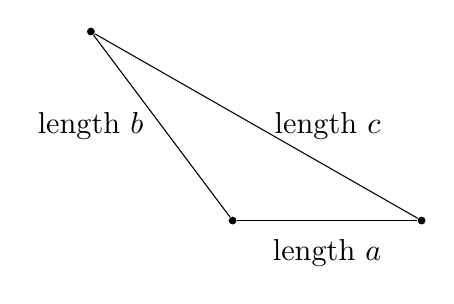
\begin{tikzpicture}[scale=1.2]
  \coordinate [circle, fill, inner sep=1pt] (a) at (1.5,0) ;
  \coordinate [circle, fill, inner sep=1pt] (b) at (0,2) ;
  \coordinate [circle, fill, inner sep=1pt] (c) at (3.5,0) ;
  \draw (a)--node[outer sep=3pt, left]{length $b$}(b) ;
  \draw (b)--node[outer sep=3pt, right]{length $c$}(c) ;
  \draw (c)--node[outer sep=3pt, below]{length $a$}(a) ;
\end{tikzpicture}

\section{Interior Angles of a Triangle}

We also talk a lot about the interior angles of a triangle:

\begin{tikzpicture}[scale=2]
  \coordinate [circle, fill, inner sep=2pt] (a) at (0,0) ;
  \coordinate [circle, fill, inner sep=2pt] (b) at (1, 2) ;
  \coordinate [circle, fill, inner sep=2pt] (c) at (3,0) ;
  \draw (a)--(b) node [outer sep=3pt, above]{$B$};
  \draw (b)--(c) node[outer sep=3pt, right]{$C$};
  \draw (c)--(a) node[outer sep=3pt, left]{$A$};
  \pic [draw, <->, "$a$", angle eccentricity=1.5] {angle = c--a--b};
  \pic [draw, <->, "$b$", angle eccentricity=1.5] {angle = a--b--c};
  \pic [draw, <->, "$c$", angle eccentricity=1.5] {angle = b--c--a};
\end{tikzpicture}

A triangle where one of the interior angles is a right angle is said to be a \emph{right triangle}:\index{right triangle}

\begin{tikzpicture}[scale=1.2]
  \coordinate [circle, fill, inner sep=2pt] (a) at (0,0) ;
  \coordinate [circle, fill, inner sep=2pt] (b) at (0,4) ;
  \coordinate [circle, fill, inner sep=2pt] (c) at (3,0) ;
  \draw (a)--(b) node [outer sep=3pt, above]{$B$};
  \draw (b)--(c) node[outer sep=3pt, right]{$C$};
  \draw (c)--(a) node[outer sep=3pt, left]{$A$};
  \pic [draw,angle eccentricity=1.5] {right angle = c--a--b};
\end{tikzpicture}

If a triangle has an obtuse interior angle, it is said to be an \emph{obtuse triangle}:\index{obtuse triange}

\begin{tikzpicture}[scale=1.2]
  \coordinate [circle, fill, inner sep=2pt] (a) at (1.5,0) ;
  \coordinate [circle, fill, inner sep=2pt] (b) at (0,2) ;
  \coordinate [circle, fill, inner sep=2pt] (c) at (3.5,0) ;
  \draw (a)--(b) node [outer sep=3pt, above]{$B$};
  \draw (b)--(c) node[outer sep=3pt, right]{$C$};
  \draw (c)--(a) node[outer sep=3pt, left]{$A$};
  \pic [draw, <->, "obtuse", angle eccentricity=1.7] {angle = c--a--b};
\end{tikzpicture}

If all three interior angles of a triangle are less than $90^\circ$, it is said to be an \emph{acute triangle}.\index{acute triangle}

The measures of the interior angles of a triangle always add up to
$180^\circ$. For example, if we know that a triangle has interior
angles of $37^\circ$ and $56^\circ$, we know that the third
interior angle is $87^\circ$.

\begin{Exercise}[title={Missing Angle}, label=missing_angle]
One interior angle of a triangle is $92^\circ$. The second angle is $42^\circ$. What is the measure of the third interior angle?
\end{Exercise}
\begin{Answer}[ref=missing_angle]
$180^\circ - (92^\circ + 42^\circ) = 46^\circ$
\end{Answer}

% Needs Diagram
How can you know that the sum of the interior angles is $180^\circ$?
Imagine that you started on the edge of a triangle and walked all the
way around to where you started. ( going
counter-clockwise.) You would turn three times to the left:

\begin{tikzpicture}[scale=1.7]
  \coordinate [circle, fill, inner sep=2pt] (a) at (1.5,0) ;  
   \node at (a) [outer sep=3pt, left]{$A$};
  \coordinate [circle, fill, inner sep=2pt] (b) at (0.5,2) ;
  \node at (b) [outer sep=3pt, above]{$B$} ;
  \coordinate [circle, fill, inner sep=2pt] (c) at (3.5,0) ;
    \node at (c)[outer sep=3pt, below]{$C$};
    
    \coordinate [circle, fill, inner sep=2pt](start) at (2.75,0);
    \node at (start)[outer sep=3pt, below]{Start};

   \coordinate (aa) at (1.75,-0.5) ;  
  \coordinate (bb) at (-0.25,2.5) ;
  \coordinate (cc) at (4.2,0) ;
  \draw [->](a)--(cc);
  \draw [->](b)--(aa);
  \draw [->](c)--(bb);
  \pic [draw, ->, "$T_C$", angle eccentricity=1.7] {angle = cc--c--b};
  \pic [draw, ->, "$T_B$", angle eccentricity=2] {angle = bb--b--a};
  \pic [draw, ->, "$T_A$", angle eccentricity=2] {angle = aa--a--c};
\end{tikzpicture}

After these three turns, you would be facing the same direction that
you started in. Thus $T_A + T_B + T_C = 360^\circ$. The
measures of the interior angles are $a$, $b$, and $c$. Notice that $a$ and
$T_A$ are supplementary. So we know that:
\begin{itemize}
\item $T_A = 180 - a$
\item $T_B = 180 - b$
\item $T_C = 180 - c$
\end{itemize}
So we can rewrite the equation above as
\begin{equation*}
  (180 - a) + (180 - b) + (180 - c) = 360^\circ
\end{equation*}
Which is equivalent to
\begin{equation*}
  a + b + c = 360^\circ
\end{equation*}

\begin{Exercise}[title={Interior Angles of a Quadrilateral}, label=interior_of_quad]
  Any four-sided polygon is a \emph{quadrilateral}. Using the same
  ``walk around the edge'' logic, what is the sum of the interior
  angles of any quadrilateral?
\end{Exercise}
\begin{Answer}[ref=interior_of_quad]
$360^\circ$
\end{Answer}


\graphicspath{{../../Chapters/pythagorean_theorem/en_US}}
\chapter{Pythagorean Theorem}

Watch's Khan Academy's Intro to the Pythagorean Theorem video at \url{https://youtu.be/AA6RfgP-AHU}.

If you have a right triangle, the edges that touch the right angle are
called \emph{the legs}.  The third edge, which is always the longest and opposite the right angle,
is known as \emph{the hypotenuse}. The Pythagorean Theorem gives us
the relationship between the length of the legs and the length of the
hypotenuse.

\begin{tikzpicture}[scale=1.2]
  \coordinate [circle, fill, inner sep=1pt] (a) at (0,0) ;
  \coordinate [circle, fill, inner sep=1pt] (b) at (0,4) ;
  \coordinate [circle, fill, inner sep=1pt] (c) at (3,0) ;
  \draw (a)--node [outer sep=3pt, left]{Length $a$}(b);
  \draw (b)--node[outer sep=3pt, right]{Length $c$}(c) ;
  \draw (c)--node[outer sep=3pt, below]{Length $b$}(a) ;
  \pic [draw, angle eccentricity=1.5] {right angle = c--a--b};
\end{tikzpicture}

The Pythagorean Theorem tells us that $a^2 + b^2 = c^2$.\index{Pythagorean theorem}

For example, if one leg has a length of 3 and the other has a length of 4, then
$a^2 + b^2 = 3^2 + 4^2 = 25$. Thus, $c^2$ must equal 25. This means you know
the hypotenuse must be of length 5. This works for any right triangle

In reality, it rarely works out to be such a tidy number. For
example, what is the length of the hypotenuse if the two legs are 3
and 6? $a^2 + b^2 = 3^2 + 6^2 = 45$.  The length of the hypotenuse is
the square root of that: $\sqrt{45} = \sqrt{9 \times 5} = 3 \sqrt{5}$,
which is approximately 6.708203932499369.

Common side lengths for these triangles are referred to as \emph{Pythagorean triples}\index{Pythagorean triples}, meaning they evaluate to a whole number. Some common examples are $(3, 4, 5)$, $(5, 12, 13)$, and $(8, 15, 17)$. Multiples of right triangles are also triangles ie. $(3, 4, 5) \implies (6, 8, 10)$, which we will touch on next chapter.

There are also angle-based right triangles, consisting of ratios of the angles of the triangles. The most common ones are $45^\circ$-$45^\circ$-$90^\circ$ and the $30^\circ$-$60^\circ$-$90^\circ$. We will discuss these further in depth, but know for now that they are vital in trigonometry, and consist of Pythagorean triples as side lengths. 

\begin{Exercise}[title={Find the Missing Length}, label=missingsides]
  What is the missing measure?
  % this formatting seems to be messed up
  \begin{multicols}{2}
Leg 1 = 6, Leg 2 = 8, Hypotenuse = ? \\(It should be a whole number.)

Leg 1 = 5, Leg 2 = ?, Hypotenuse = 13 \\(It should be a whole number.)
  
Leg 1 = ?, Leg 2 = 15, Hypotenuse = 17 \\(It should be a whole number.)

Leg 1 = 3, Leg 2 = 3, Hypotenuse = ? \\(It is an irrational number. Give the exact answer and then use a calculator to get an approximation.)
\end{multicols}
\end{Exercise}
\begin{Answer}[ref=missingsides]
  10 because $6^2 + 8^2 = 10^2$

  12 because $5^2 + 12^2 = 13^2$

  8 because $8^2 + 15^2 = 17^2$

  $3\sqrt{2} \approx 4.24$ because $3^2 + 3^2 = \left(3 \sqrt{2}\right)^2$
\end{Answer}


\section{Distance between Points}

What is the distance between these two points?\index{distance using Pythagorean theorem}

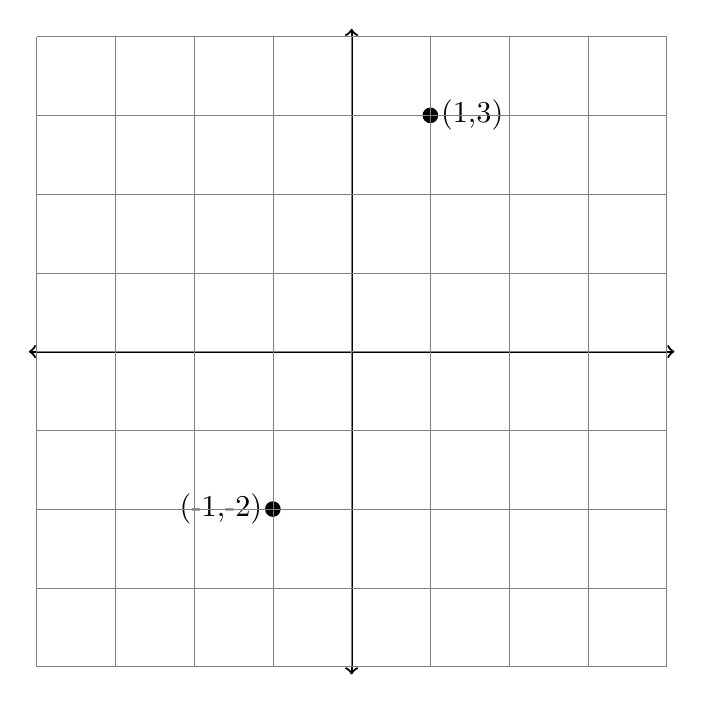
\begin{tikzpicture}
  % axis
  \draw[thick, <->] (0, -4.1) -- (0, 4.1);
  \draw[thick, <->] (-4.1, 0) -- (4.1, 0);
  \coordinate [circle, fill, inner sep=2pt] (a) at (-1,-2) ;
  \coordinate [circle, fill, inner sep=2pt] (b) at (1,3) ;
  \node [left] at (a) {(-1,-2)};
  \node [right] at (b) {(1,3)};
  % grid
  \draw[help lines, step = 1cm] (-4, -4) grid (4, 4);
  
\end{tikzpicture}

We can draw a right triangle and use the Pythagorean Theorem:

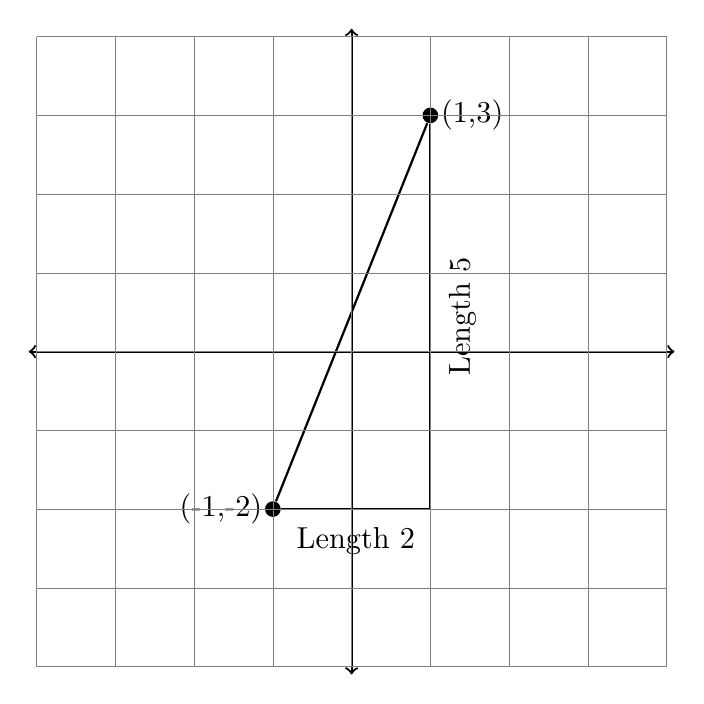
\begin{tikzpicture}
  % axis
  \draw[thick, <->] (0, -4.1) -- (0, 4.1);
  \draw[thick, <->] (-4.1, 0) -- (4.1, 0);
  \coordinate [circle, fill, inner sep=2pt] (a) at (-1,-2) ;
  \coordinate [circle, fill, inner sep=2pt] (b) at (1,3) ;
    \node [left] at (a) {(-1,-2)};
  \node [right] at (b) {(1,3)};
  \coordinate (c) at (1, -2);

  \draw [thick] (a) -- (b);
  \draw [thick] (a) -- node[outer sep = 3pt, below]{Length 2}(c);
  \draw [thick] (c) -- node[rotate=90, outer sep = 3pt, below]{Length 5}(b);
  \draw[help lines, step = 1cm] (-4, -4) grid (4, 4);
 
\end{tikzpicture}


The distance between the two points is $\sqrt{2^2 + 5^2} = \sqrt{29}
\approx 5.385165$. In other words, you square the change in $x$ and add it to
the square of the change in $y$. The distance is the square root of
that sum.

\section{Distance in 3 Dimensions}

What if the point is in three-dimensional space?  For example, you move 2
meters East, 8 meters North, and 4 meters up in the air. How far are
you from where you started?  You just square each, sum them, and take the square root:
$\sqrt{2^2 + 8^2 + 4^2} = \sqrt{84} = 2\sqrt{21} \approx 9.165$ meters.\index{distance!in 3 dimensions}

\begin{tikzpicture}
  \draw [thick, ->] (0,0,0) -- (9,0,0) node[outer sep = 1pt, right]{North} ; 
  \draw [thick, ->]  (0,0,0) -- (0,3,0) node[outer sep = 1pt, above]{Up} ; 
  \draw [thick, ->] (0,0,0) -- (0,0,4) node[outer sep = 1pt, below]{East} ; 

    \draw [dashed]  (8,0,0) -- node[outer sep = 1pt, right]{2}  (8,0,2); 

  \draw [dashed]  (0,0,2) -- node[outer sep = 1pt, below]{8} (8,0,2); 
  \draw [dashed]  (8,0,2) -- node[outer sep = 1pt, right]{4} (8,4,2); 
  \draw [thick]  (0,0,0) --  (8,4,2) node[circle, fill, inner sep=2pt]{}; 
  \node [left] at (5, 2.7, 1){$\sqrt{2^2 + 8^2 + 4^2} \approx 9.165$};

\end{tikzpicture}

This leads us to a formal definition of the distance formula:
\[
d = \sqrt{(x_2 - x_1)^2 + (y_2 - y_1)^2}
\]
Or in 3D space:
\[
d = \sqrt{(x_2 - x_1)^2 + (y_2 - y_1)^2 + (z_2 - z_1)^2}
\]

\graphicspath{{../../Chapters/congruence/en_US}}
\chapter{Congruence}
% Add: simple triangles
%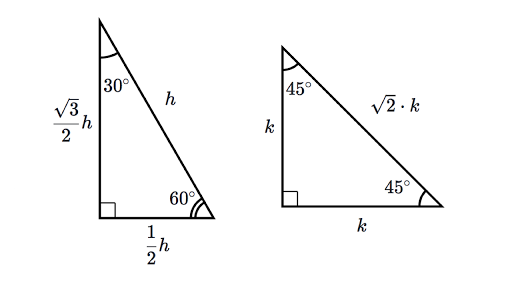
\includegraphics[width=0.8\textwidth]{KA_Special_Triangles.png}
Look at this picture of two geometric figures.

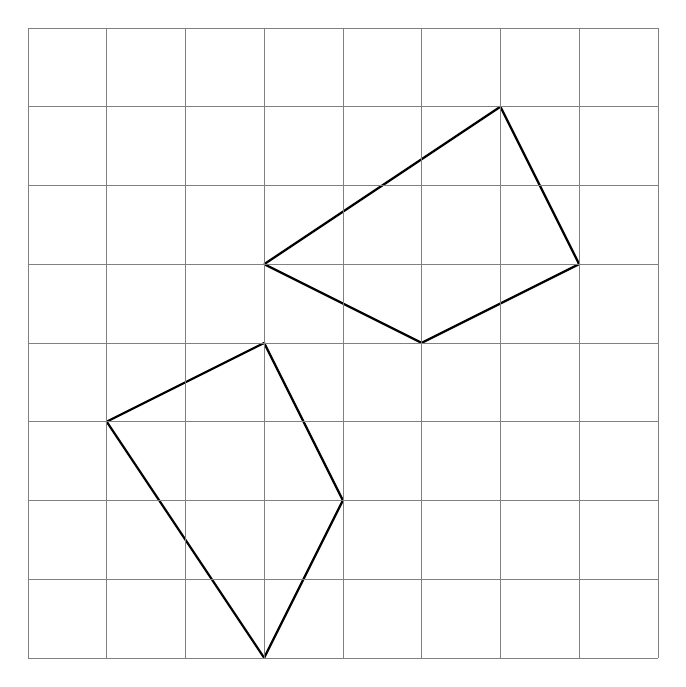
\begin{tikzpicture}
 
  	\draw [thick] (-1,-4) --  (0, -2);
	\draw [thick] (0,-2) --  (-1, 0) ;
	\draw [thick] (-1,0) --  (-3, -1); 
	\draw [thick] (-3,-1) --  (-1, -4);
	
	\draw [thick] (-1,1) --  (1, 0);
	\draw [thick] (1,0) --  (3, 1) ;
	\draw [thick] (3,1) --  (2, 3); 
	\draw [thick] (2,3) --  (-1, 1);

  \draw[help lines, step = 1cm] (-4, -4) grid (4, 4);
 
\end{tikzpicture}

They are the same shape, right? If you cut one out with scissors, it
would lay perfectly on top of the other. In geometry, we say they are
\emph{congruent}.

What is the official definition of ``congruent''? 
Two geometric figures are congruent if you can transform one into the other using
only rigid transformations. 

You might be wondering now, what are rigid transformations?
A transformation is \emph{Rigid} if it doesn't change the distances
between the points or the measure of the angles between the lines, they
form. These are all rigid transformations:
\begin{itemize}
\item Translations
\item Rotations
\item Reflections 
\end{itemize}

Once again imagine cutting out one figure with scissors and trying to match it with the second figure, your actions are rigid transformations:
\begin{itemize}
\item Translations - sliding the cutout left and right and up and down
\item Rotations	- rotating the cutout clockwise and counterclockwise
\item Reflection - flipping the piece of paper over
\end{itemize}

A transformation is rigid if it is some combination of translations, rotations, and reflections.

\section{Triangle Congruency}

If the sides of two triangles have the same length, the triangles must be congruent:

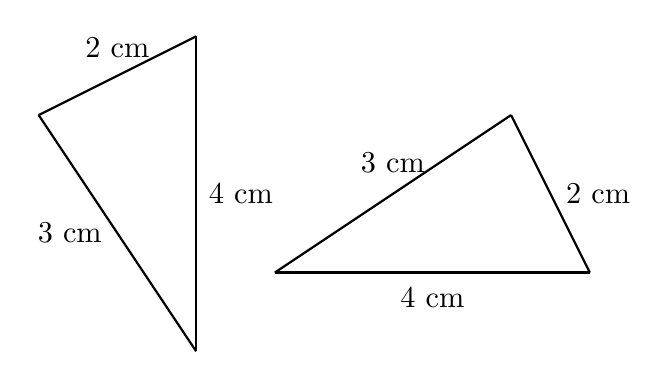
\begin{tikzpicture} 
  	\draw [thick] (-2,0) -- node[outer sep = 1pt, right]{4 cm}  (-2, 4) ;
	\draw [thick] (-2,4) --  node[outer sep = 3pt, above]{2 cm} (-4, 3); 
	\draw [thick] (-4,3) --  node[outer sep = 2pt, left]{3 cm} (-2, 0);
	
	\draw [thick] (-1,1) --  node[outer sep = 2pt, below]{4 cm}  (3, 1) ;
	\draw [thick] (3,1) --  node[outer sep = 2pt, right]{2 cm} (2, 3); 
	\draw [thick] (2,3) --  node[outer sep = 4pt, above]{3 cm} (-1, 1);
\end{tikzpicture}

To be precise, the Side-Side-Side Congruency Test says that two triangles are
congruent if three sides in one triangle are the same length as the
corresponding sides in the other. We usually refer to this as the SSS test.
% Explain with a^2 + b^2 = c^2

Note that two triangles with all three angles equal are not necessarily congruent.
For example, here are two triangles with the same interior angles, but they are
different sizes:

\begin{tikzpicture}
  \coordinate [circle, fill, inner sep=1pt] (a1) at (0,0) ;
  \coordinate [circle, fill, inner sep=1pt] (b1) at (4,0) ;
  \coordinate [circle, fill, inner sep=1pt] (c1) at (3,2) ;
  
   \coordinate [circle, fill, inner sep=1pt] (a2) at (5,0) ;
  \coordinate [circle, fill, inner sep=1pt] (b2) at (11,0) ;
  \coordinate [circle, fill, inner sep=1pt] (c2) at (9.5,3) ;
        \draw (a1) --   (b1);
        \draw (b1) -- (c1);
        \draw (c1)--  (a1);
        \pic [draw, "$63^\circ$", angle eccentricity=1.5] {angle = c1--b1--a1};
        \pic [draw, "$34^\circ$", angle eccentricity=2.0] {angle = b1--a1--c1};
        \pic [draw, "$83^\circ$", angle eccentricity=1.5] {angle = a1--c1--b1};

       \draw (a2) --  (b2);
        \draw (b2) -- (c2);
        \draw (c2)--  (a2);
        \pic [draw, "$63^\circ$", angle eccentricity=1.5] {angle = c2--b2--a2};
        \pic [draw, "$34^\circ$", angle eccentricity=2.0] {angle = b2--a2--c2};
        \pic [draw, "$83^\circ$", angle eccentricity=1.5] {angle = a2--c2--b2};

\end{tikzpicture}

These triangles are not congruent, but they are \emph{similar}. Meaning
 they have the same shape, but are not necessarily the same
size.

Therefore, if you know two angles of a triangle, you can calculate the third. So it makes sense
to say ``If two triangles have two angles that are equal, they are
similar triangles.''  And if two similar triangles have one side that
is equal in length, they must be the same size -- so they are
congruent. Thus, the Side-Angle-Angle Congruency Test says that
two triangles are congruent if two angles and one side match.

What if you know that two triangles have two sides that are the same
length and that the angle between them is also equal?

\begin{tikzpicture}
  \coordinate [circle, fill, inner sep=1pt] (a1) at (0,0) ;
  \coordinate [circle, fill, inner sep=1pt] (b1) at (4,0) ;
  \coordinate [circle, fill, inner sep=1pt] (c1) at (3,2) ;
  
  \coordinate [circle, fill, inner sep=1pt] (a2) at (5,0) ;
  \coordinate [circle, fill, inner sep=1pt] (b2) at (9,0) ;
  \coordinate [circle, fill, inner sep=1pt] (c2) at (8,2) ;
  
  \draw (a1) --  node[outer sep = 0.5pt, below]{4}  (b1);
  \draw [dashed] (b1) -- (c1);
  \draw (c1)--  node[outer sep = 5pt, above]{3.5} (a1);
  \pic [draw, "$34^\circ$", angle eccentricity=2.0] {angle = b1--a1--c1};

  \draw (a2) --  node[outer sep = 0.5pt, below]{4}  (b2);
  \draw [dashed] (b2) -- (c2);
  \draw (c2)--  node[outer sep = 5pt, above]{3.5} (a2);
  \pic [draw, "$34^\circ$", angle eccentricity=2.0] {angle = b2--a2--c2};
\end{tikzpicture}

Yes, they must be congruent. This is the Side-Angle-Size Congruency Test.

What if the angle isn't the one between the two known sides? If it is
a right angle, you can be certain the two triangles are congruent.
(How do I know? Because the Pythagorean Theorem tells us that we can
calculate the length of the third side. There is only one possibility,
thus all three sides must be the same length.)

\begin{tikzpicture}
  \coordinate [circle, fill, inner sep=1pt] (a1) at (0,0) ;
  \coordinate [circle, fill, inner sep=1pt] (b1) at (4,0) ;
  \coordinate [circle, fill, inner sep=1pt] (c1) at (4,2) ;
  
   \coordinate [circle, fill, inner sep=1pt] (a2) at (5,0) ;
  \coordinate [circle, fill, inner sep=1pt] (b2) at (9,0) ;
  \coordinate [circle, fill, inner sep=1pt] (c2) at (9,2) ;
        \draw (a1) --  node[outer sep = 0.5pt, below]{3.5}  (b1);
        \draw [dashed] (b1) -- (c1);
        \draw (c1)--  node[outer sep = 5pt, above]{4} (a1);
        \pic [draw] {right angle = a1--b1--c1};

        \draw (a2) --  node[outer sep = 0.5pt, below]{3.5}  (b2);
        \draw [dashed] (b2) -- (c2);
        \draw (c2)--  node[outer sep = 5pt, above]{4} (a2);
        \pic [draw] {right angle = a2--b2--c2};
\end{tikzpicture}

In this case, the third side of each triangle must be $\sqrt{4^2 - 3.5^2} \approx 1.9$.

What if the know angle is less than $90^\circ$? \emph{The triangles
  are not necessarily congruent.} For example, let's say that there are
two triangles with sides of length 5 and 7 and that the corresponding
angle (at the end of the side of length 7) on each is $45^\circ$. Two
different triangles satisfy this:

\begin{tikzpicture}
  \coordinate [circle, fill, inner sep=1pt] (a1) at (0,0) ;
  \coordinate [circle, fill, inner sep=1pt] (b1) at (7,0) ;
  \coordinate [circle, fill, inner sep=1pt] (c1) at (4,3) ;
  \coordinate [circle, fill, inner sep=1pt] (a2) at (8,0) ;
  \coordinate [circle, fill, inner sep=1pt] (b2) at (15,0) ;
  \coordinate [circle, fill, inner sep=1pt] (c2) at (11,4) ;
  \draw (a1) --  node[outer sep = 0.5pt, below]{7}  (b1);
  \draw [dashed] (b1) -- (c1);
  \draw (c1)--  node[outer sep = 5pt, above]{5}(a1);
  \pic [draw, "$45^\circ$", angle eccentricity=1.5] {angle = c1--b1--a1};
  \draw (a2) --  node[outer sep = 0.5pt, below]{7}  (b2);
  \draw [dashed] (b2) -- (c2);
  \draw (c2)--  node[outer sep = 5pt, above]{5} (a2);
  \pic [draw, "$45^\circ$", angle eccentricity=1.5] {angle = c2--b2--a2};
\end{tikzpicture}

Let's see this another way by laying one triangle on top of the other:

\begin{tikzpicture}
  \coordinate [circle, fill, inner sep=1pt] (a1) at (0,0) ;
  \coordinate [circle, fill, inner sep=1pt] (b1) at (7,0) ;
  \coordinate [circle, fill, inner sep=1pt] (c1) at (4,3) ;
  \coordinate [circle, fill, inner sep=1pt] (c2) at (3,4) ;
  \coordinate (d) at (2,5);
  \coordinate (e) at (3.5,3.5);

  \draw (a1) --  node[outer sep = 0.5pt, below]{7}  (b1);
  \draw [dashed,->] (b1) -- (d);
  \draw [dashed] (a1) -- (e);
  \draw (c1)--  node[outer sep = 5pt, below]{5}(a1);
  \draw (c2)--  node[outer sep = 5pt, above]{5}(a1);
  \pic [draw, "$45^\circ$", angle eccentricity=1.5] {angle = c1--b1--a1};
   \pic [draw, angle radius=8] {right angle = b1--e--a1};
\end{tikzpicture}


So there is \emph{not} a general Side-Side-Angle Congruency Test.

Here, then, is the list of common congruency tests:
\begin{itemize}
\item Side-Side-Side: All three sides have the same measure
\item Side-Angle-Angle: Two angles and one side have the same measure
\item Side-Angle-Side: Two sides and the angle between them have the same measure
\item Side-Side-Right: They are right triangles and have two sides have the same measure
\end{itemize}

\begin{Exercise}[title={Congruent Triangles}, label=con_triangles]
  Ted is terrible at drawing triangles: he always draws them exactly
  the same. Fortunately, he has marked these diagrams with the sides
  and angles that he measured. For each pair of triangles, write if
  you know them to be congruent and which congruency test proves
  it. For example:

\begin{tikzpicture}[scale=0.7]
  \coordinate [circle, fill, inner sep=1pt] (a1) at (0,1) ;
  \coordinate [circle, fill, inner sep=1pt] (b1) at (5,0) ;
  \coordinate [circle, fill, inner sep=1pt] (c1) at (4,2) ;
  
  \coordinate [circle, fill, inner sep=1pt] (a2) at (6,1) ;
  \coordinate [circle, fill, inner sep=1pt] (b2) at (11,0) ;
  \coordinate [circle, fill, inner sep=1pt] (c2) at (10,2) ;
  \draw (a1) --  node[outer sep = 0.5pt, below]{3.5}  (b1);
  \draw (b1) -- node[outer sep = 2pt, right]{4} (c1);
  \draw (c1)--  node[outer sep = 2pt, above]{} (a1);
  \pic [draw,  "$120^\circ$", angle eccentricity=2.0] {angle = c1--b1--a1};

  \draw (a2) --  node[outer sep = 0.5pt, below]{3.5}  (b2);
  \draw  (b2) -- node[outer sep = 2pt, right]{4} (c2);
  \draw (c2) -- node[outer sep = 2pt, above]{} (a2);
  \pic [draw,  "$120^\circ$",, angle eccentricity=2.0] {angle = c2--b2--a2};
\end{tikzpicture}

  (These drawings are clearly not accurate, but you are told the measurements are.) The answer is ``Congruent by the Side-Angle-Side test.''

  \begin{multicols}{2}

\begin{tikzpicture}[scale=0.6]
  \coordinate [circle, fill, inner sep=1pt] (a1) at (0,1) ;
  \coordinate [circle, fill, inner sep=1pt] (b1) at (5,0) ;
  \coordinate [circle, fill, inner sep=1pt] (c1) at (4,2) ;
  
  \coordinate [circle, fill, inner sep=1pt] (a2) at (6,1) ;
  \coordinate [circle, fill, inner sep=1pt] (b2) at (11,0) ;
  \coordinate [circle, fill, inner sep=1pt] (c2) at (10,2) ;
  \draw (a1) --  node[outer sep = 0.5pt, below]{3.5}  (b1);
  \draw (b1) -- node[outer sep = 2pt, right]{} (c1);
  \draw (c1)--  node[outer sep = 2pt, above]{6} (a1);
  \pic [draw,  "$90^\circ$", angle eccentricity=2.0] {angle = c1--b1--a1};

  \draw (a2) --  node[outer sep = 0.5pt, below]{3.5}  (b2);
  \draw  (b2) -- node[outer sep = 2pt, right]{} (c2);
  \draw (c2) -- node[outer sep = 2pt, above]{6} (a2);
  \pic [draw,  "$90^\circ$",, angle eccentricity=2.0] {angle = c2--b2--a2};
\end{tikzpicture}

\hspace{3cm}

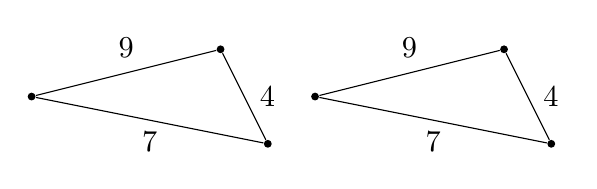
\begin{tikzpicture}[scale=0.6]
  \coordinate [circle, fill, inner sep=1pt] (a1) at (0,1) ;
  \coordinate [circle, fill, inner sep=1pt] (b1) at (5,0) ;
  \coordinate [circle, fill, inner sep=1pt] (c1) at (4,2) ;
  
  \coordinate [circle, fill, inner sep=1pt] (a2) at (6,1) ;
  \coordinate [circle, fill, inner sep=1pt] (b2) at (11,0) ;
  \coordinate [circle, fill, inner sep=1pt] (c2) at (10,2) ;
  \draw (a1) --  node[outer sep = 0.5pt, below]{7}  (b1);
  \draw (b1) -- node[outer sep = 2pt, right]{4} (c1);
  \draw (c1)--  node[outer sep = 2pt, above]{9} (a1);

  \draw (a2) --  node[outer sep = 0.5pt, below]{7}  (b2);
  \draw  (b2) -- node[outer sep = 2pt, right]{4} (c2);
  \draw (c2) -- node[outer sep = 2pt, above]{9} (a2);
\end{tikzpicture}


\begin{tikzpicture}[scale=0.6]
  \coordinate [circle, fill, inner sep=1pt] (a1) at (0,1) ;
  \coordinate [circle, fill, inner sep=1pt] (b1) at (5,0) ;
  \coordinate [circle, fill, inner sep=1pt] (c1) at (4,2) ;
  
  \coordinate [circle, fill, inner sep=1pt] (a2) at (6,1) ;
  \coordinate [circle, fill, inner sep=1pt] (b2) at (11,0) ;
  \coordinate [circle, fill, inner sep=1pt] (c2) at (10,2) ;
  \draw (a1) --  node[outer sep = 0.5pt, below]{7}  (b1);
  \draw (b1) -- node[outer sep = 2pt, right]{} (c1);
  \draw (c1)--  node[outer sep = 2pt, above]{} (a1);
  \pic [draw,  "$35^\circ$",, angle eccentricity=2.0] {angle = c1--b1--a1};
  \pic [draw,  "$62^\circ$",, angle eccentricity=2.0] {angle = b1--a1--c1};

  \draw (a2) --  node[outer sep = 0.5pt, below]{7}  (b2);
  \draw  (b2) -- node[outer sep = 2pt, right]{} (c2);
  \draw (c2) -- node[outer sep = 2pt, above]{} (a2);
  \pic [draw,  "$35^\circ$",, angle eccentricity=2.0] {angle = c2--b2--a2};
  \pic [draw,  "$62^\circ$",, angle eccentricity=2.0] {angle = b2--a2--c2};

\end{tikzpicture}

\hspace{3cm}


\begin{tikzpicture}[scale=0.6]
  \coordinate [circle, fill, inner sep=1pt] (a1) at (0,1) ;
  \coordinate [circle, fill, inner sep=1pt] (b1) at (5,0) ;
  \coordinate [circle, fill, inner sep=1pt] (c1) at (4,2) ;
  
  \coordinate [circle, fill, inner sep=1pt] (a2) at (6,1) ;
  \coordinate [circle, fill, inner sep=1pt] (b2) at (11,0) ;
  \coordinate [circle, fill, inner sep=1pt] (c2) at (10,2) ;
  \draw (a1) --  node[outer sep = 0.5pt, below]{8}  (b1);
  \draw (b1) -- node[outer sep = 2pt, right]{6} (c1);
  \draw (c1)--  node[outer sep = 2pt, above]{} (a1);
  \pic [draw,  "$28^\circ$",, angle eccentricity=2.0] {angle = b1--a1--c1};

  \draw (a2) --  node[outer sep = 0.5pt, below]{8}  (b2);
  \draw  (b2) -- node[outer sep = 2pt, right]{6} (c2);
  \draw (c2) -- node[outer sep = 2pt, above]{} (a2);
  \pic [draw,  "$28^\circ$",, angle eccentricity=2.0] {angle = b2--a2--c2};

\end{tikzpicture}


\end{multicols}
\end{Exercise}

\begin{Answer}[ref=con_triangles]
\begin{multicols}{2}
Congruent by the Side-Side-Right Congruency Test.

Congruent by the Side-Side-Side Congruency Test.

Congruent by the Side-Angle-Angle Congruency Test.

We don't know if they are congruent. The measured angle is not between the measured sides.

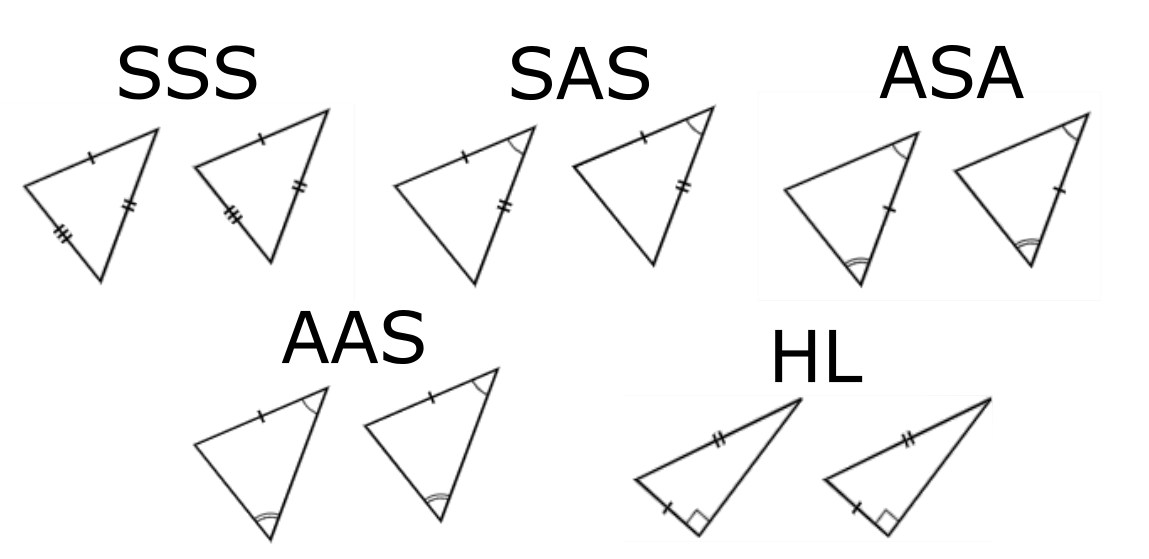
\includegraphics[width=0.8\textwidth]{Triangle_Congruence.png}
\end{multicols}

\end{Answer}




\graphicspath{{../../Chapters/parallel_perpendicular/en_US}}
\chapter{Parallel and Perpendicular}

Two vectors are said to be parallel if they have the same or opposite
direction. In simpler terms, if two vectors are pointing in the same
direction (even if their magnitudes differ), they are considered
parallel. For example, imagine you have a vector representing the
direction and speed of a car moving north. If you have another vector
representing the direction and speed of a different car also moving
north, these vectors are parallel.\index{parallel}

On the other hand, if two vectors point in completely opposite
directions, they are still considered parallel. For instance, if one
vector represents a car moving north and the other represents a car
moving south, these vectors are parallel but in opposite directions.

Perpendicular vectors, as the name suggests, are vectors that
intersect each other at a right angle, forming a 90-degree angle. If
we imagine a sheet of paper, drawing a horizontal vector and a
vertical vector on that paper would create perpendicular vectors. In
this case, the horizontal vector represents left-right direction,
while the vertical vector represents up-down direction. Perpendicular
vectors are often seen in geometric shapes, such as squares and
rectangles, where their sides intersect at right angles.\index{perpendicular}

A fundamental property of perpendicular vectors is that their dot
product is zero. The dot product is a mathematical operation that
measures the extent to which two vectors align with each other. When
two vectors are perpendicular, their dot product is always zero. This
property provides a useful tool for determining whether two given
vectors are perpendicular.

Understanding parallel and perpendicular vectors is essential in
various areas of mathematics and physics. For example, in geometry,
knowledge of perpendicular vectors helps us determine whether lines
are perpendicular or parallel. In physics, vectors can represent
forces, velocities, or displacements, and identifying parallel or
perpendicular vectors aids in analyzing motion and forces acting on
objects.

In summary, parallel vectors have the same or opposite direction,
while perpendicular vectors intersect at a right angle. Recognizing
these relationships between vectors enables us to solve problems
involving geometry, physics, and many other fields. As you delve
deeper into the exciting world of vectors, keep an eye out for
parallel and perpendicular relationships, as they often hold valuable
insights and solutions.

\graphicspath{{../../Chapters/circles/en_US}}
\chapter{Circles}

A circle is the set of points $(x, y)$ that are a particular distance $r$ from a
particular point $(x_c, y_c)$.  We say that $r$ is the
\newterm{radius} and $(x_c, y_c)$ is the \newterm{center}

\begin{tikzpicture}
    \filldraw [sdkblue] (1,2) circle (2pt) node[anchor=west]{$(x_c, y_c)$};
    \filldraw [sdkblue] (2,4.82842712474619) circle (2pt) node[anchor=west]{
    $(x, y)$};
    \draw [sdkblue,dashed](1,2) -- (2,4.82842712474619) node[midway,anchor=
    west] {$r$};
    \draw [sdkblue](1,2) circle (3);
    \draw [stealth-stealth](-2.5,0)--(4.5,0);
    \draw [stealth-stealth](0,-1.5)--(0,5.5);
\end{tikzpicture}

\begin{mdframed}[style=important, frametitle={Area and Radius}]

  If the radius of a circle is $r$, the area of its interior ($a$) is given 
  by \index{circle!area of}

  $$a = \pi r^2$$

\end{mdframed}

\begin{Exercise}[title={Area of a Circle}, label=area_of_circle]

  The paint you have says ``One liter covers 6 square meters.''

  You are painting the top of a circular table with a radius of 3 meters.

  How much paint will you need?
  
\end{Exercise}
\begin{Answer}[ref=area_of_circle]

  The table has a radius of 3 meters.

  So the area of its top is $3^2 \pi \approx 28.27$.

  $$ 28.27 \text{ square meters }\left(\frac{1 \text{ liter }}{6 \text{ square 
  meters }} \right) = 4.72 \text{ liters }$$ 
  
\end{Answer}


Note that a circle lives in a particular plane. The points $(x, y, z)$ that 
are a particular distance $r$ from a particular point $(x_c, y_c, z_c)$ are a 
sphere:

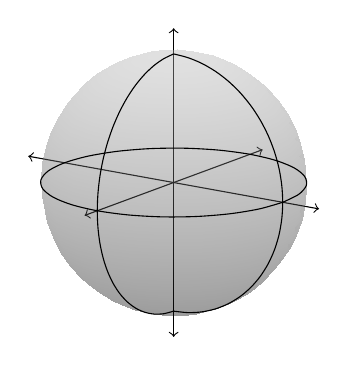
\begin{tikzpicture}
  \begin{axis}[
    view={35}{15},
    unit vector ratio=1 1 1,
    ticks = none,
    axis lines=middle,
    ymin=-3.5,
    ymax=3.5,
    xmax=4.0,
    xmin=-4.0,
    zmin=-3.6,
    zmax=3.6,
    x axis line style=<->,
    y axis line style=<->,
    z axis line style=<->,
    clip=false
    ]
    \addplot3[surf,shader=interp,domain=0:360,y domain=-90:90, opacity=0.4,
    colormap={blackwhite}{color=(black) color=(black!30)}] ({3 * cos(y) * 
    cos(x)},
    {3 *  cos(y) * sin(x)},{3 * sin(y)});
    \addplot3[samples y=0,domain=0:360,smooth]({3*cos(x)}, {3*sin(x)}, 0.0);
    \addplot3[samples y=0,domain=-180:0,smooth](0, {3*sin(x)}, {3*cos(x)});
    \addplot3[samples y=0,domain=0:180,smooth]({3*sin(x)}, 0, {3*cos(x)});
  \end{axis}
\end{tikzpicture}

The distance all the way across the middle of a circle (or a sphere) is its
\newterm{diameter}.  The diameter is always twice the radius.

For the rest of the chapter, we are talking about circles, points, and
lines \textit{in a plane}.

\begin{mdframed}[style=important, frametitle={Circumference and Diameter}]

  The circumference ($c$) of a circle is the distance around the circle. If the
  diameter is $d$, \index{circumference}

  $$c = \pi d$$

\end{mdframed}

\begin{Exercise}[title={Circumference}, label=circumference]

  Using a tape measure, you figure out that the circumference of a tree in your
  yard is 64 cm.

  Assuming the trunk is basically circular,  what is its diameter?
  
\end{Exercise}
\begin{Answer}[ref=circumference]

  The diameter is $$\frac{c}{\pi} = \frac{64}{\pi} \approx 20.37 \text{ 
  centimeters}$$
  
\end{Answer}
\begin{Exercise}[title={Splitting a Pie}, label=pie_splitting]

  A pie has a radius of 13 cm.  7 friends all want equal sized wedges.  You 
  have a tape measure.

  How many centimeters will each outer crust be?

\end{Exercise}
\begin{Answer}[ref=pie_splitting]

  The circumference of the pie is $26 \pi \approx 81.7$ centimenters.
  
  The length of the crust for each piece would be about $\frac{81.7}{7} = 11.7$
  cm.

  
\begin{tikzpicture}
    \filldraw [black] (0,0) circle (2pt);
    \draw [black](0,0) circle (3);
    \foreach \x in {0,...,6}
    \draw [dashed] (0,0) -- ({3 * cos(\x * 51.428571428571429)}, {3 * sin(\x 
    * 51.428571428571429)});
    \draw [sdkblue,very thick] (3, 0) arc (0:51.43:3) node [midway, anchor=east] 
    {11.7 cm};
    \node at (1.0, 1.5)  {13 cm};
\end{tikzpicture}
\end{Answer}



\begin{mdframed}[style=important, frametitle={Length of an Arc}]

If you have two points $a$ and $b$ on a circle, the ray from the
center through $a$ and the ray from the center through $b$ form an
angle.  If $\theta$ is the angle in radians and $r$ is the radius of
the circle, the distance from $a$ to $b$ on the circle is $r \theta$.

\begin{tikzpicture}
    \filldraw [black] (0,0) circle (2pt) node[anchor=west]{Center};
    \filldraw [sdkblue] (-1,2.82842712474619) circle (2pt) node[anchor=west]{$b$};
    \filldraw [sdkblue] (2.12132,2.12132) circle (2pt) node[anchor=east]{$a$};
    \draw [sdkblue,dashed,->](0,0) -- (-1.2,3.394112549695428);
    \draw [sdkblue,dashed,->](0,0) -- (2.4, 2.4) node[midway,anchor=east]{$r$};
    \draw [black](0,0) circle (3);
    \draw [sdkblue,very thick] (2.12132,2.12132) arc (45:109.47:3) node [midway, 
    anchor=south] {$r \theta$};
    \draw [sdkblue, <->] (0.707,0.707) arc (45:109.47:1) node [midway, 
    anchor=south]{$\theta$};
\end{tikzpicture}

\end{mdframed}

\begin{Exercise}[title={Arc Length}, label=arc_length]

You have been asked to find the radius of a very large cylindrical tank.
You have a tape measure, but it is only 15 meters long and doesn't
reach all the way around the tank.

However, you have a compass.  So you stick one end of the tape measure
to the side of the tank and measure the orientation of the wall at
that point.  Then you walk the 15 meters and measure the orientation of the 
wall there.

You find that 15 meters represents 72 degrees of arc.

What is the radius of the tank in meters?
  
\end{Exercise}
\begin{Answer}[ref=arc_length]

  $$72 \text{ degrees } \left(\frac{2\pi \text{ radians }}{360 \text{ degrees }
  }\right) \approx 1.2566 \text{ radians }$$

  $$15 = 1.2566r$$

  $$r = 11.94 \text{ meters}$$
  
\begin{tikzpicture}
    \filldraw [black] (0,0) circle (2pt);
    \draw [black](0,0) circle (3);
    \draw [dashed] (0,0) -- ({3 * cos(72)}, {3 * sin(72)});
    \draw [dashed] (0,0) -- (3, 0);
    \draw [sdkblue,very thick] (3,0) arc (0:72:3) node [midway, anchor=east] 
    {15 m};
    \draw [sdkblue, <->] (1,0) arc (0:72:1) node [midway, anchor=east]{$72^
    \circ$ = 1.2566 rad};
    \node at (0.0, 1.6)  {11.94 m};
\end{tikzpicture}
\end{Answer}

\section{Tangents}

A line that is \newterm{tangent} to a circle touches it at exactly one point:

\begin{tikzpicture}
    \filldraw [black] (0,0) circle (2pt);
    \draw [dashed, black](0,0) circle (3);
    \filldraw [sdkblue] (2.121, 2.121) circle (2pt);
    \draw [sdkblue, thick] (6.243, -2) -- (0, 4.243);
\end{tikzpicture}

The tangent line is always perpendicular to the radius to the point of tangency:

\begin{tikzpicture}
  \filldraw [black] (0,0) circle (2pt);
  \draw [dashed, black](0,0) circle (3);
  \filldraw [sdkblue] (2.121, 2.121) circle (2pt);
  \draw [sdkblue, thick] (0,0) -- (2.121, 2.121);
  \draw [black] (1.9, 1.9) -- (2.121, 1.679) -- (2.342,1.9);
  \draw [sdkblue, thick] (6.243, -2) -- (0, 4.243);
\end{tikzpicture}


\begin{Exercise}[title={Painting a Comet}, label=painting_comet]
  
  You have been asked to paint a comet and its tail in yellow on the floor of a 
  gymnasium.

  A liter of yellow paint covers 6 square meters.

  First you draw a circle with a radius of 3 meters.  Then you mark a
  point $D$ on the floor 7 meters from the center of the circle.  Then
  you draw two tangent lines that pass through $D$.

  You use a protractor to measure the angle at which the tangent lines meet: about 
  $51^\circ$
  
  \begin{tikzpicture}
    \filldraw [sdkblue] (0,0) circle (2pt);
    \filldraw [black] (7,0) circle (2pt);
    \draw [sdkblue,dashed] (0,0) -- (3,0) node [midway, anchor=south] {3 m};
    \draw [sdkblue,dashed] (3,0) -- (7,0) node [midway, anchor=south] {4 m};
    \draw [sdkblue,dashed, ->] (5.5,0) arc (180:154.6:1.5) node [midway, 
    anchor=west]{$51^\circ$};
    \draw [sdkblue,dashed, ->] (5.5,0) arc (180:205.4:1.5);
    \draw [black,thick] (7,0) -- ({3 * cos(64.62)}, {3 * sin(64.62)});
    \draw [black,thick] (7,0) -- ({3 * cos(-64.62)}, {3 * sin(-64.62)});
    \filldraw [black] ({3 * cos(64.62)}, {3 * sin(64.62)}) circle (2pt);
    \filldraw [black] ({3 * cos(-64.62)}, {3 * sin(-64.62)}) circle (2pt);
    \filldraw [sdkblue] (3, 0) circle (2pt);
    \draw [sdkblue,dashed] ({3 * cos(-64.62)}, {3 * sin(-64.62)}) arc 
    (-64.62:64.62:3);
    \draw [black,thick] ({3 * cos(64.62)}, {3 * sin(64.62)}) arc 
    (64.62:295.38:3);
  \end{tikzpicture}

  Before you paint the area contained by the circle and the two
  tangent lines, how much paint will you need?
    

\end{Exercise}
\begin{Answer}[ref=painting_comet]

  The trick here is to take advantage of the fact that the tangent is 
  perpendicular to the radius to make right triangles:

  \begin{tikzpicture}
    \coordinate (a) at ({3 * cos(64.62)}, {3 * sin(64.62)});
    \coordinate (b) at ({3 * cos(-64.62)}, {3 * sin(-64.62)});
    \filldraw [sdkblue] (0,0) circle (2pt);
    \filldraw [black] (7,0) circle (2pt);
    \draw [black,thick] (0,0) -- (a) node [midway, anchor=east] {3m};
    \draw [black,thick] (0,0) -- (b) node [midway, anchor=east] {3m};
    \draw [black,thick] (0,0) -- (7,0) node [midway, anchor=south] {7 m};
    \draw [sdkblue,dashed, <->] (5.5,0) arc (180:154.6:1.5) node [midway, 
    anchor=west]{$25.5^\circ$};
    \draw [sdkblue,dashed, <->] (5.5,0) arc (180:205.4:1.5) node [midway, 
    anchor=west]{$25.5^\circ$};
    \draw [sdkblue,dashed, <->] (1.5,0) arc (0:64.5:1.5) node [midway, 
    anchor=west]{$64.5^\circ$};
    \draw [sdkblue,dashed, <->] (1.5,0) arc (0:-64.5:1.5) node [midway, 
    anchor=west]{$64.5^\circ$};
    \draw [black,thick] (7,0) -- (a);
    \draw [black,thick] (7,0) -- (b);
    \filldraw [black] (a) circle (2pt);
    \filldraw [black] (b) circle (2pt);
    \draw [black,thick] (a) arc (64.62:295.38:3);
  \end{tikzpicture}

  The wedge has radius 3 and represents $360 - 2(64.5) = 231^\circ \approx 4.03 
  \text{ radians}$.

  We are finding the area of this piece:
  
  \begin{tikzpicture}
    \coordinate (a) at ({3 * cos(64.62)}, {3 * sin(64.62)});
    \coordinate (b) at ({3 * cos(-64.62)}, {3 * sin(-64.62)});
    \filldraw [sdkblue] (0,0) circle (2pt);
    \draw [black,thick] (0,0) -- (a) node [midway, anchor=west] {3m};
    \draw [black,thick] (0,0) -- (b);
    \draw [sdkblue,dashed, <->] ({1.5 * cos(64.62)}, {1.5 * sin(64.62)}) arc 
    (64.5:295.5:1.5) node [midway]{4.03 rad};
    \filldraw [black] (a) circle (2pt);
    \filldraw [black] (b) circle (2pt);
    \draw [black,thick] (a) arc (64.62:295.38:3);
  \end{tikzpicture}

  The area of this piece is $(4.03)(3^2) = 36.27$ square meters.

  If a right triangle has a hypotenuse of 7m and one leg is 3m, the
  other leg is $\sqrt{7^2 - 3^2} = 2 \sqrt{10} \approx 6.3$ m.

    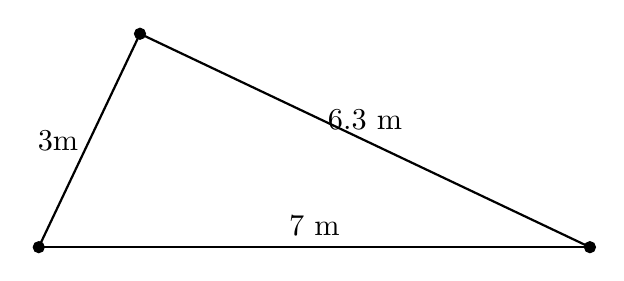
\begin{tikzpicture}
    \coordinate (a) at ({3 * cos(64.62)}, {3 * sin(64.62)});
    \filldraw [black] (7,0) circle (2pt);
    \filldraw [black] (0,0) circle (2pt);
    \draw [black,thick] (0,0) -- (a) node [midway, anchor=east] {3m};
    \draw [black,thick] (0,0) -- (7,0) node [midway, anchor=south] {7 m};
    \draw [black,thick] (7,0) -- (a) node [midway, anchor=south] {6.3 m};
    \filldraw [black] (a) circle (2pt);
  \end{tikzpicture}

  
  A right triangle with legs of 3m and 6.3m has an area of 9.45 square meters.

  There are two of them, so the total area is $36.27 + 2(18.9) = 74.07$ square 
  meters.

  Six square meters per liter, so you need $\frac{74.07}{6} = 12.35$ liters of 
  paint.

\end{Answer}

\section{Radians and circles}
Previously, you learned that angles can be measured in degrees and radians. A 
circle is $360^o$ (see figure \ref{fig:circledeg}). 

\begin{figure}[htbp]
\centering
\begin{tikzpicture}
        \begin{polaraxis}[axis lines = none, clip = false]
    \draw[black](0,0) -- (0, 3);
    \draw[black, dashed] (0,0) -- (180, 3);
    \addplot[blue, thick, domain = 0:360, samples = 200]{2.5};
    \addplot[red, domain = 0:175]{1};
    \draw[red, -latex](175, 1) -- (180,1);
    \addplot[red, domain = 180:355]{1};
    \draw[red, -latex] (355, 1) -- (360, 1);
    \node[] at (90, 1.5) {$\theta_1 = 180^\circ$};
    \node[] at (270, 1.5) {$\theta_2 = 180^\circ$};
    \end{polaraxis}
    \end{tikzpicture}
    \caption{The total internal angle of a circle is $\theta_1 + \theta_2 = 
    360^\circ$}
    \label{fig:circledeg}
\end{figure}

This means a circle is also $2\pi$ radians:
$$360^\circ \cdot \frac{\pi}{180^\circ} = 2\pi$$

You may have been wondering: why is it that there are $\pi$ radians in a 
$180^\circ$ angle? A radian is defined such that one radian is the angle at the 
center of a circle which defines an arc of the circumference equal to the 
radius of the circle (see figure \ref{fig:oneradian}). 

\begin{figure}[htbp]
\centering
\begin{tikzpicture}
        \begin{polaraxis}[axis lines = none, ymin = 0, ymax = 3, 
	clip = false]
 \addplot[blue, thick, domain = 0:360, samples = 300] {2.5};
 \addplot[red, thick, domain = 0:57.3] {2.5};
 \draw[red, thick](0,0) -- (0, 2.5);
 \draw[red, thick] (0,0) -- (57.3, 2.5);
 \addplot[red, domain = 0:57.3]{0.5};
 \addplot[black, domain = 0:57.3]{2.75};
 \draw[black](0,2.7) -- (0,2.8);
 \draw[black] (57.3, 2.7) -- (57.3, 2.8);
 \node[rotate = -60] at (27.5, 2.9) {\small length $= r$};
 \node[] at (27.5, 1) {\small $\theta = 1$};
    \end{polaraxis}
    \end{tikzpicture}
    \caption{When the center angle is 1 radian, the length of the arc is equal 
    to the radius of the circle}
    \label{fig:oneradian}
\end{figure} 

This makes it very straightforward to find the lengths of arcs if we know the 
center angle in radians. The arc length is just $\theta r$, where $\theta$ is 
the center angle in radians. 
%%%%%%%%%%%%%%%%%%%%%%%%%%%%%%%%%
%% Bookfooter.tex by Aaron Hillegass
%% Nov 8, 2020

\appendix

\chapter{Answers to Exercises}
\shipoutAnswer

\bibliography{references}

\printindex

\end{document}